\documentclass[11pt]{article}
\usepackage{float}
\usepackage{graphicx}
\usepackage{tabularx}
\usepackage{adjustbox}
\usepackage{amsmath,amssymb,trimclip,adjustbox}
%\usepackage[utf8]{inputenc}
%\usepackage[T1]{fontenc}
\usepackage{textcomp}
\usepackage{booktabs}
\newcommand{\Csh}{C\includegraphics{hash-symbol}}
\begin{document}
	\begin{titlepage}
		\begin{center}
			\Large{Warsaw University of Technology's}\\
			\Large{Faculty of Mathematics and Information Science}\\
			[0.3in]
			\begin{figure}[H]
				\centering
				\includegraphics[width=0.4\linewidth, height=0.25\textheight]{./media/uni_logo.jpeg}
				\label{Figure:f04}
			\end{figure}
			\Large{\bfseries Knowledge Representation and Reasoning}\\
			[0.3in]
			\Large{\bfseries Project number 2:}\\
			\Large{\bfseries Deterministic Action With Cost}\\
			\Large{\bfseries Supervisor: Dr Anna Radzikowska}\\
			[0.3in]
			\Large{\bfseries Test case Documentation}\\
			[0.3in]
			\textsc{\Large{Created By}\\
				Rishabh Jain,
				Rahul Tomer,
				Kuldeep Shankar,\\ 
				Alaa Abboushi,
				Haran Dev Murugan,\\
				Bui Tuan Anh.\\}
		\end{center}	
	\end{titlepage}
	\tableofcontents
	\newpage
	\section{Introduction}\label{sec:intro}
	This document is to Show the test cases of the application that is used to implement the language $\mathcal{A}$ with cost statements. The Languages assumptions are as follows.
	Let C2 be a class of dynamic systems satisfying the following assumptions:
	\begin{enumerate}
		\item Inertia law
		\item Complete information about all actions and fluent. 
		\item Only Determinism
		\item Only sequential actions are allowed.
		\item Characterizations of actions:\begin{itemize}
			\item Precondition represented by set of literals(a fluent or its negation);if a precondition does not hold, the action is executed but with empty effect
			\item Postcondition (effect of an action) represented by a set of literals.
			\item Cost $k \in N $ of an action, actions with empty effects cost 0. Each action has a fixed cost, if it leads to non-empty effects. 
		\end{itemize}
		\item Effects of an action depends on the state where the action starts.
		\item All actions are performed in all states.
		\item Partial description of any state of the system are allowed.
		\item No constraints are defined.	 
	\end{enumerate}
	\section{Examples}\label{sec:Examples}
	\subsubsection{Description}\label{par:p101}
	Andrew wants to travel by his car to a place. Travelling costs him 50\$ when there is fuel in car tank. Travelling costs him 50\$ when there is fuel in reserve. When there is no fuel in any of it, Andrew can fuy fuel. Fuel costs him 40\$
	\subsubsection{Representation}\label{par:p201}
	Fluents: F = \{fuel, reserve\}\\
	Actions: Ac = \{buy, travel\}\\
	Costs: K = \{40, 50\}\\
	\\
	initially  fuel; \\
	initially $\neg$reserve; \\
	travel causes $\neg$fuel if fuel, reserve; \\
	travel causes $\neg$reserve if $\neg$fuel, reserve;\\
	travel causes $\neg$fuel if fuel, $\neg$reserve\\
	travel costs 50; \\
	buy causes fuel if $\neg$ fuel,reserve;\\
	buy causes fuel if $\neg$ fuel,$\neg$reserve;\\
	buy causes reserve if  fuel,$\neg$reserve;\\
	buy costs 40; \\
	\subsubsection{Calculation}\label{par:p301}\par
	$\sum$ = $\lbrace$ $\sigma_{0}$,$\sigma_{1}$,$\sigma_{2}$,$\sigma_{3}$ $\rbrace$\\ \\
	$\sigma_{0}$ = $\lbrace$ fuel, $\neg$reserve $\rbrace$ \indent $\sigma_{1}$ = $\lbrace$ $\neg$fuel, $\neg$reserve $\rbrace$\\
	$\sigma_{2}$ = $\lbrace$ $\neg$fuel, reserve $\rbrace$ \indent 	
	$\sigma_{3}$ = $\lbrace$ fuel,reserve $\rbrace$
	\\
	$\Psi$(buy, $\sigma_{0}$)=$\sigma_{3}$\\ 
	$\Psi$(travel, $\sigma_{0}$)=$\sigma_{1}$\\
	\(\Gamma\)(buy, $\sigma_{0}$) = 40\\
	\(\Gamma\)(travel, $\sigma_{0}$) = 50\\
	\\
	$\Psi$(buy, $\sigma_{1}$)=$\sigma_{0}$\\ 
	$\Psi$(travel, $\sigma_{1}$)=$\sigma_{1}$\\
	\(\Gamma\)(buy, $\sigma_{1}$) = 40\\
	\(\Gamma\)(travel, $\sigma_{1}$) = 0\\
	\\
	$\Psi$(buy, $\sigma_{2}$)=$\sigma_{3}$\\ 
	$\Psi$(travel, $\sigma_{2}$)=$\sigma_{1}$\\
	\(\Gamma\)(buy, $\sigma_{2}$) = 40\\
	\(\Gamma\)(travel, $\sigma_{2}$) = 50\\
	\\
	$\Psi$(buy, $\sigma_{3}$)=$\sigma_{3}$\\ 
	$\Psi$(travel, $\sigma_{3}$)=$\sigma_{2}$\\
	\(\Gamma\)(buy, $\sigma_{3}$) = 0\\
	\(\Gamma\)(travel, $\sigma_{3}$) = 50\\
	\subsubsection{Graph}\label{par:p401}
	\begin{figure}[H]
		\centering
		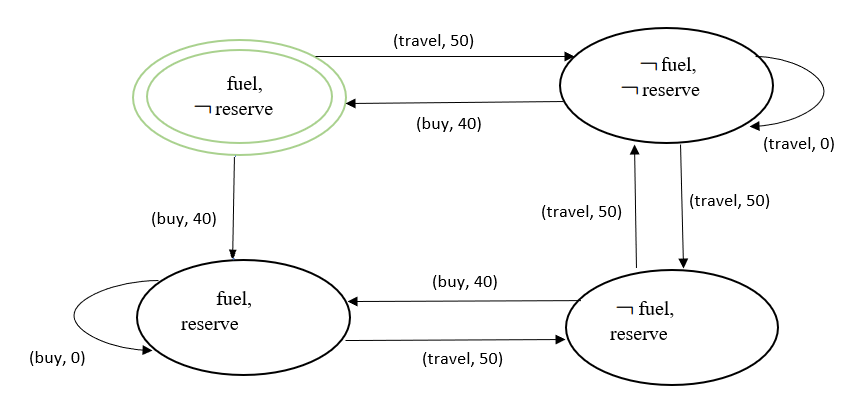
\includegraphics[width=6in,height=3in]{./media/ex01.png}
		\label{Figure:f01}
		\caption{Example 01}
	\end{figure}
	\subsubsection{Queries}
	reserve holds after (travel, travel, buy, buy): True\\
	fuel holds after (buy, travel, buy,travel): False\\
	\\
	150 sufficient for (travel, travel, buy, travel): True\\
	90 sufficient for (buy, travel, buy): False\\
	\subsubsection*{Test Images}\label{par:501}
	\begin{figure}[H]
		\centering
		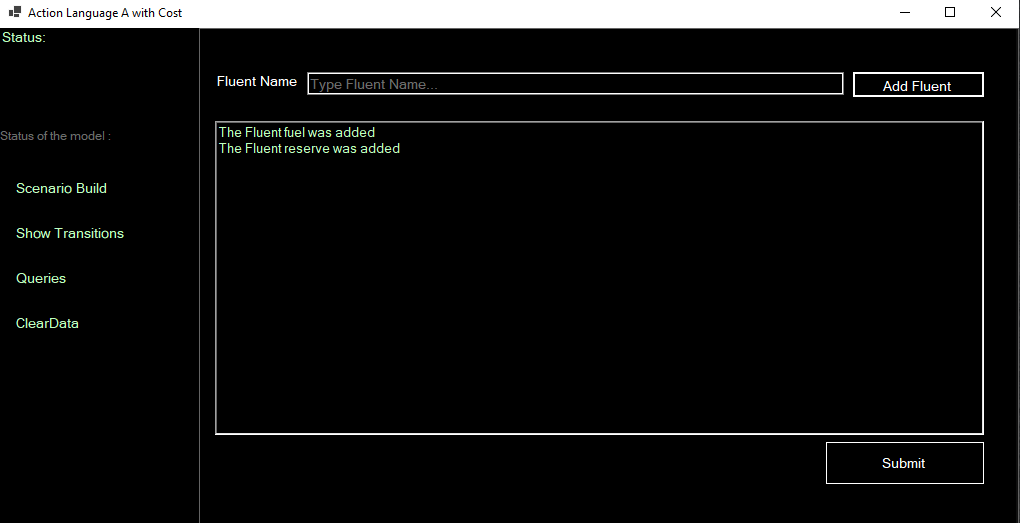
\includegraphics[width=6in,height=3in]{./testImages/Example1/img1.png}
		\label{Figure:f01.1}
		\caption{Add Fluents}
	\end{figure}
	\begin{figure}[H]
		\centering
		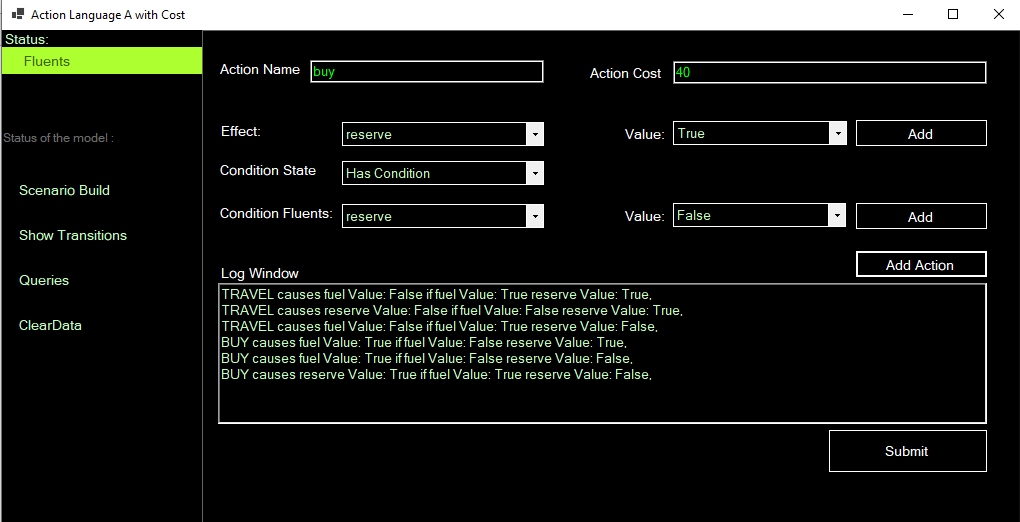
\includegraphics[width=6in,height=3in]{./testImages/Example1/img2.png}
		\label{Figure:f01.2}
		\caption{Add Actions}
	\end{figure}
	\begin{figure}[H]
		\centering
		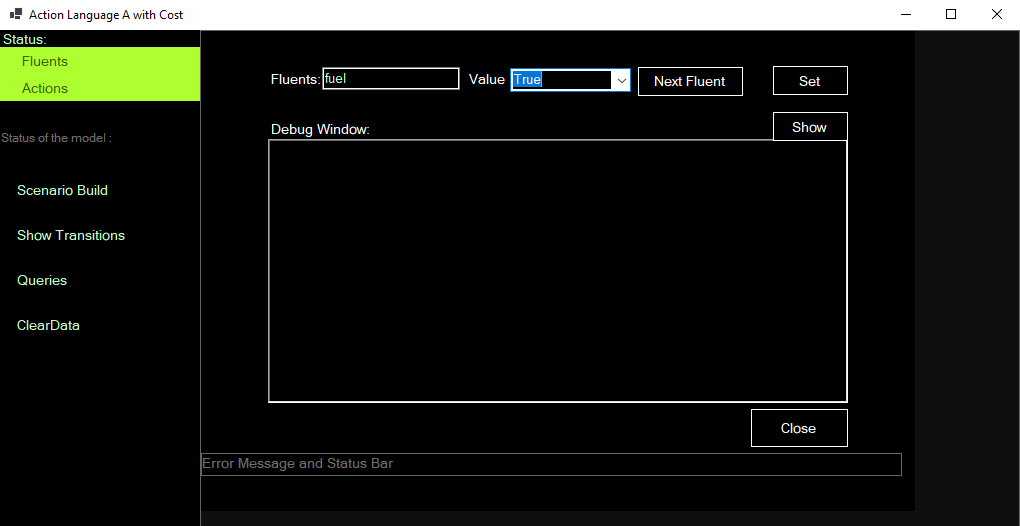
\includegraphics[width=6in,height=3in]{./testImages/Example1/img3.png}
		\label{Figure:f01.3}
		\caption{Set Initial State fluents}
	\end{figure}
	\begin{figure}[H]
		\centering
		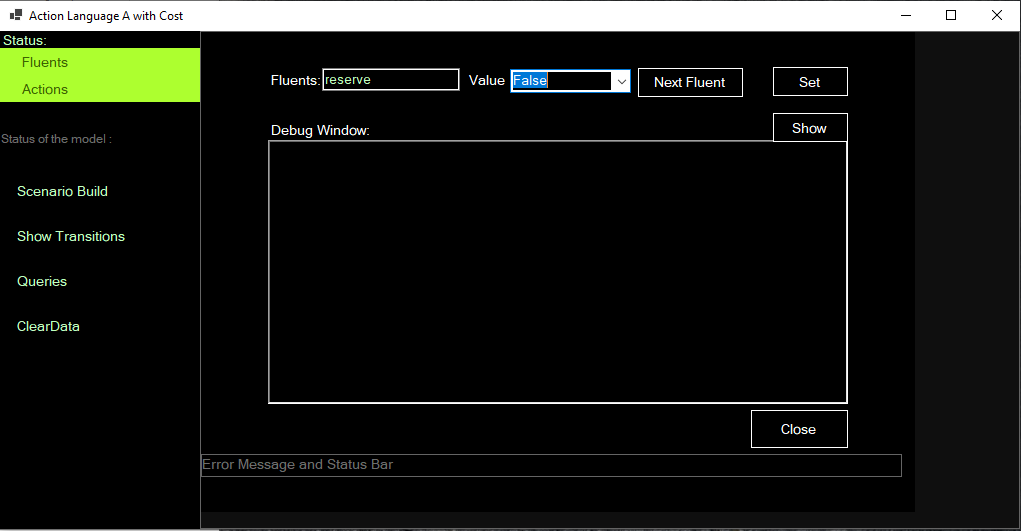
\includegraphics[width=6in,height=3in]{./testImages/Example1/img4.png}
		\label{Figure:f01.4}
		\caption{Set Initial state}
	\end{figure}
	\begin{figure}[H]
		\centering
		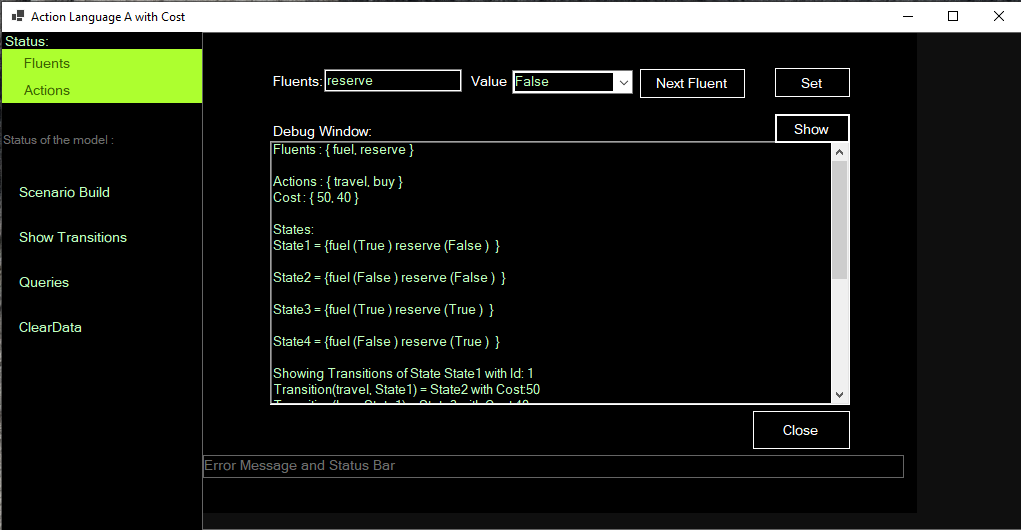
\includegraphics[width=6in,height=3in]{./testImages/Example1/img5.png}
		\label{Figure:f01.5}
		\caption{Show Transitions}
	\end{figure}
		\begin{figure}[H]
		\centering
		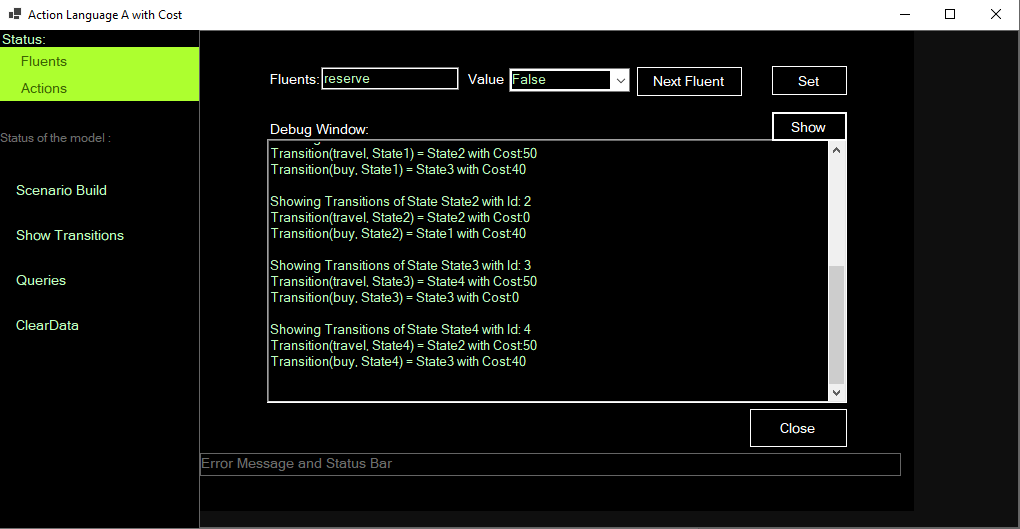
\includegraphics[width=6in,height=3in]{./testImages/Example1/img6.png}
		\label{Figure:f01.6}
		\caption{Show Transition contd..}
	\end{figure}
		\begin{figure}[H]
		\centering
		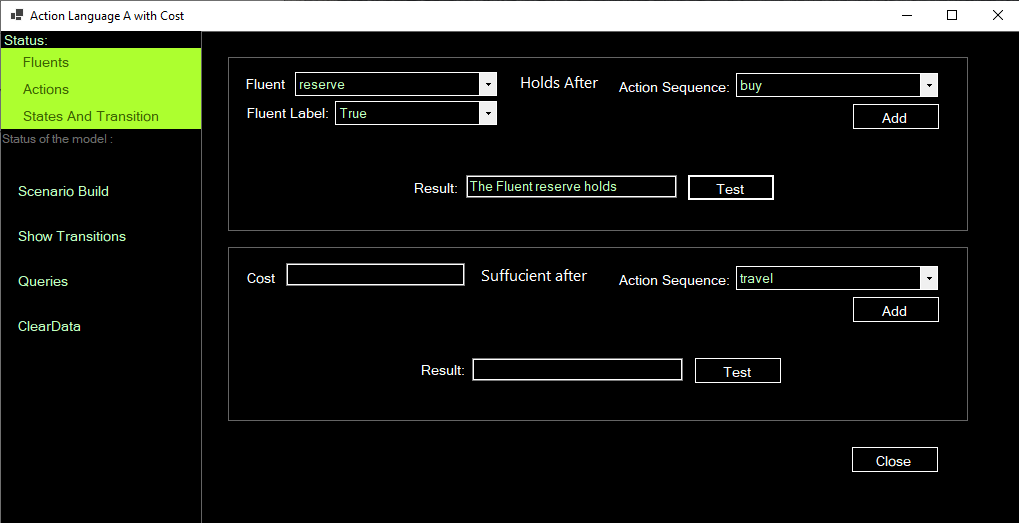
\includegraphics[width=6in,height=3in]{./testImages/Example1/img7.png}
		\label{Figure:f01.7}
		\caption{Queries(Fluents)}
	\end{figure}
	\begin{figure}[H]
		\centering
		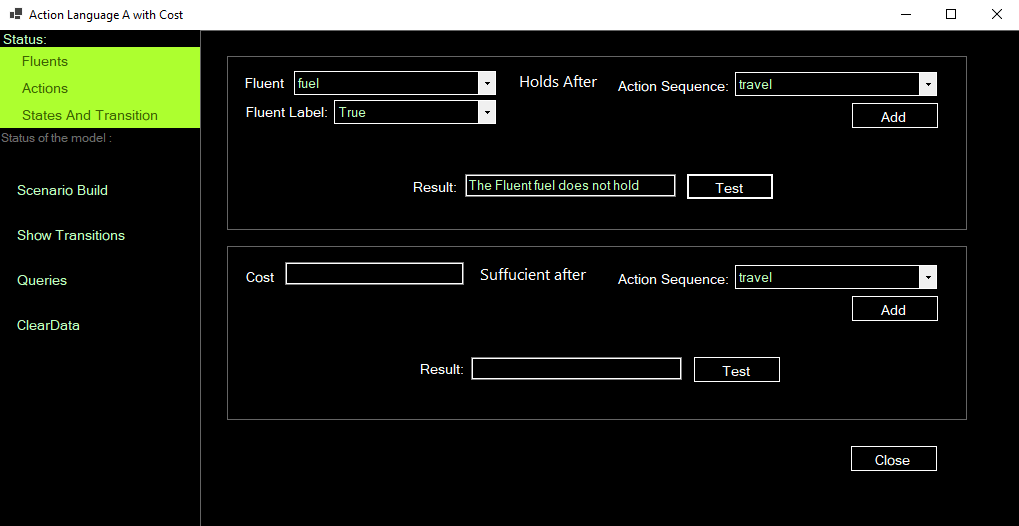
\includegraphics[width=6in,height=3in]{./testImages/Example1/img8.png}
		\label{Figure:f01.8}
		\caption{Queries(Fluents)}
	\end{figure}
	\begin{figure}[H]
		\centering
		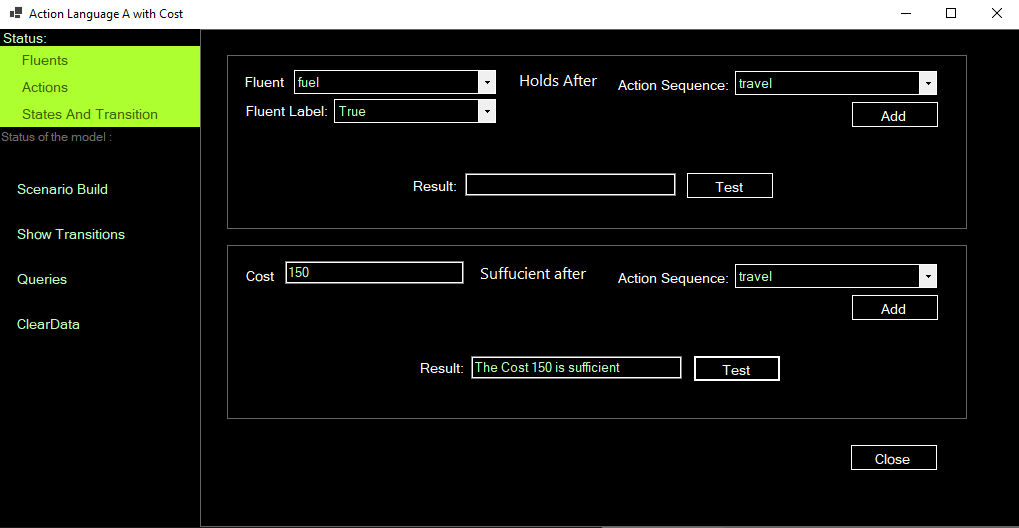
\includegraphics[width=6in,height=3in]{./testImages/Example1/img9.png}
		\label{Figure:f01.8}
		\caption{Queries(Cost)}
	\end{figure}
	\begin{figure}[H]
		\centering
		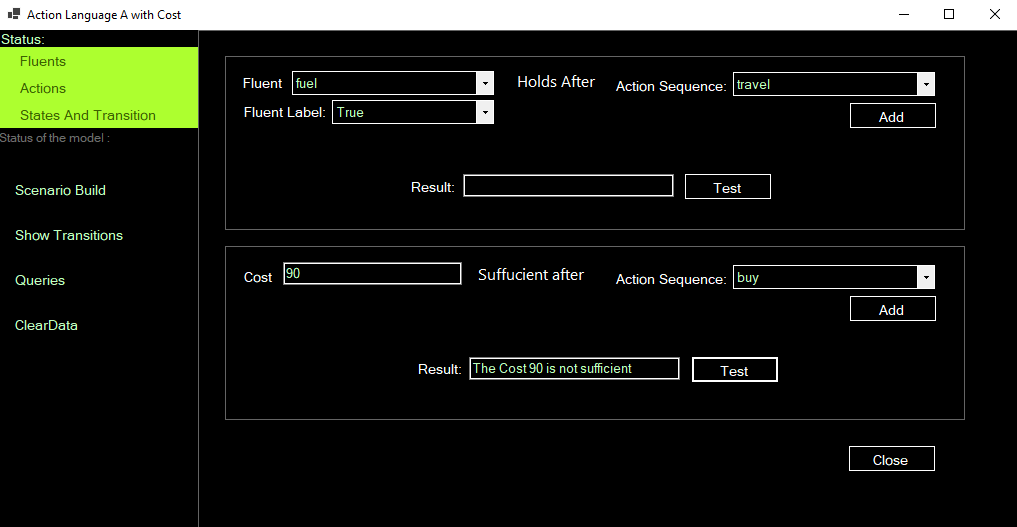
\includegraphics[width=6in,height=3in]{./testImages/Example1/img10.png}
		\label{Figure:f01.8}
		\caption{Queries(Cost)}
	\end{figure}

		
	\subsection{Example 02}\label{example:ex02}
	\subsubsection{Description}\label{par:p102}
	John visits a painter to buy a specific painting. The cost of painting is 200\$ if its available in the shop. But if painting is not available then John needs to order a new one to be painted and will buy once its available.Order costs 50\$ At any time only one copy of painting is available and another one to be ordered once sold. 
	
	\subsubsection{Representation:}\label{par:p202}
	\indent 
	Fluents: F = \{available, sold\}\\
	Actions: Ac = \{buy, order\}\\
	Costs: K = \{200, 50\}\\
	initially ¬available;\\
	initially ¬sold;\\
	buy causes sold if available;\\
	buy causes ¬available;\\
	buy costs 200\$;\\
	order causes available if ¬available;\\
	order costs 50\$; \\
	
	\subsubsection{Calculation:}\label{par:p302}
	\indent \\
	$ \sum $ = $ \{ $ $ \sigma _{0}$, $ \sigma _{1}$, $ \sigma _{2}$, $ \sigma _{3}$$ \} $ \\
	$ \sigma _{0}$ = $ \{ $ ¬available, ¬sold$ \} $ \\
	$ \sigma _{1}$ = $ \{ $ available, ¬sold$ \} $ \\
	$ \sigma _{2}$ = $ \{ $ ¬available, sold$ \} $ \\
	$ \sigma _{3}$ = $ \{ $ available, sold$ \} $ \\
	\\
	\(  \Psi  \)  (buy, $ \sigma $0) = $ \sigma $0\\
	\(  \Psi  \)  (order, $ \sigma $0) = $ \sigma $1\\
	\(\Gamma\)(buy, $\sigma_{0}$) = 0\\
	\(\Gamma\)(order, $\sigma_{0}$) = 50\\
	\\
	\(  \Psi  \)  (buy $ \sigma $1) = $ \sigma $2\\
	\(  \Psi  \)  (order, $ \sigma $1) = $ \sigma $1\\
	\(\Gamma\)(buy, $\sigma_{1}$) = 200\\
	\(\Gamma\)(order, $\sigma_{1}$) = 0\\
	\\
	\(  \Psi  \)  (buy, $ \sigma $2) = $ \sigma $2\\
	\(  \Psi  \)  (order, $ \sigma $2) = $ \sigma $3\\
	\(\Gamma\)(buy, $\sigma_{2}$) = 0\\
	\(\Gamma\)(order, $\sigma_{2}$) = 50\\
	\\
	\(  \Psi  \)  (buy, $ \sigma $3) = $ \sigma $2\\
	\(  \Psi  \)  (order, $ \sigma $3) = $ \sigma $3\\
	\(\Gamma\)(buy, $\sigma_{3}$) = 200\\
	\(\Gamma\)(order, $\sigma_{3}$) = 0\\

	\subsubsection{Graph}\label{par:p402}
	\begin{figure}[H]
		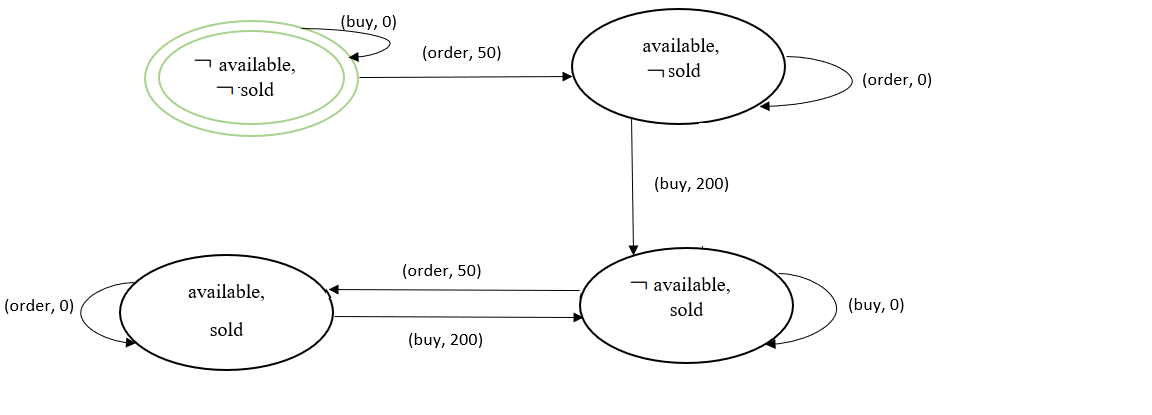
\includegraphics[width=1.2\linewidth, height=0.4\textheight]{./media/example2_graph.png}
		\label{Figure:f02}
		\caption{Example 02}
	\end{figure}
	\subsubsection{Queries}
	available holds after (buy, order, buy, order): True\\
	available holds after (buy, order, buy): False\\
	\\
	275 sufficient for (buy, order, order, buy): True\\
	190 sufficient for (order, buy, buy, order): False\\
	\subsubsection*{Test Images}\label{par:502}
	\begin{figure}[H]
		\centering
		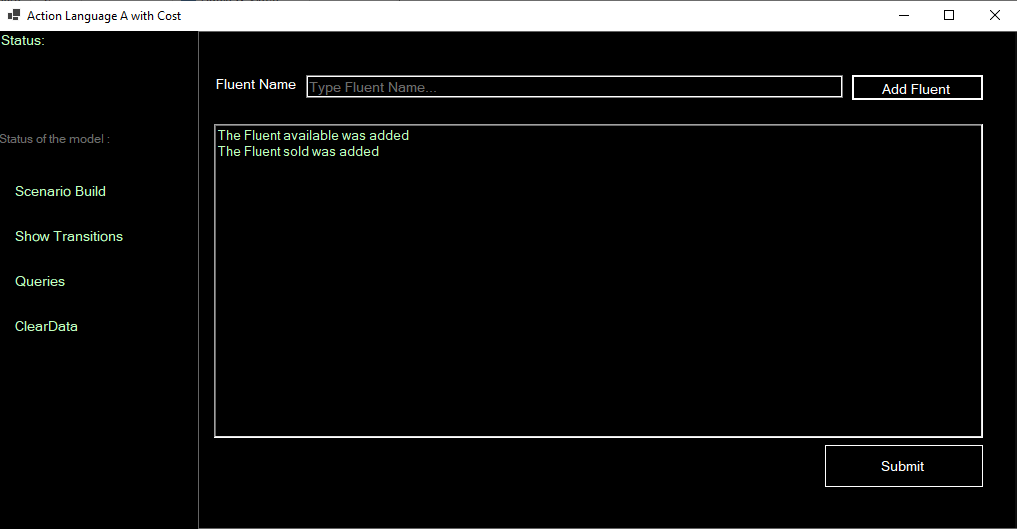
\includegraphics[width=6in,height=3in]{./testImages/Example2/img1.png}
		\label{Figure:f02.1}
		\caption{Add Fluents}
	\end{figure}
	\begin{figure}[H]
		\centering
		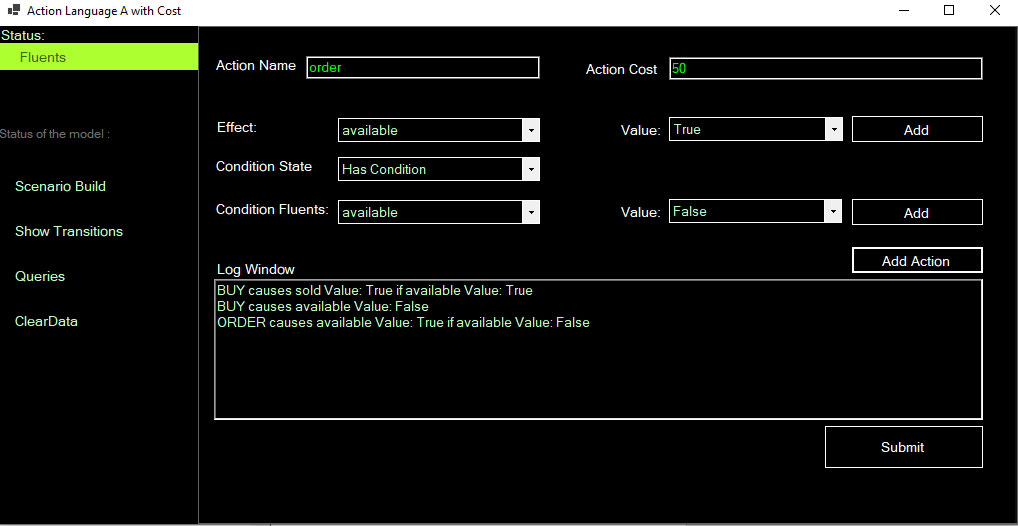
\includegraphics[width=6in,height=3in]{./testImages/Example2/img2.png}
		\label{Figure:f02.2}
		\caption{Add Actions}
	\end{figure}
	\begin{figure}[H]
		\centering
		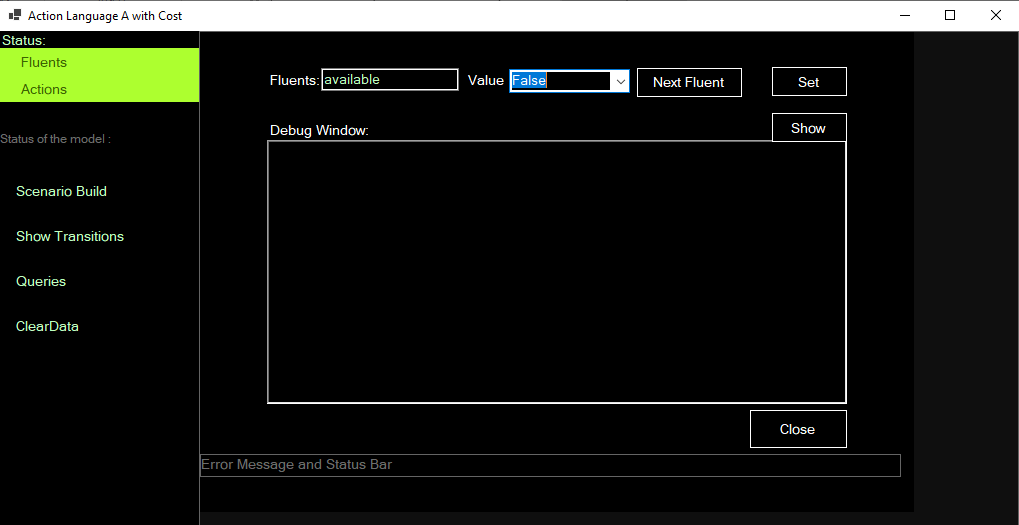
\includegraphics[width=6in,height=3in]{./testImages/Example2/img3.png}
		\label{Figure:f02.3}
		\caption{Set Initial State fluents}
	\end{figure}
	\begin{figure}[H]
		\centering
		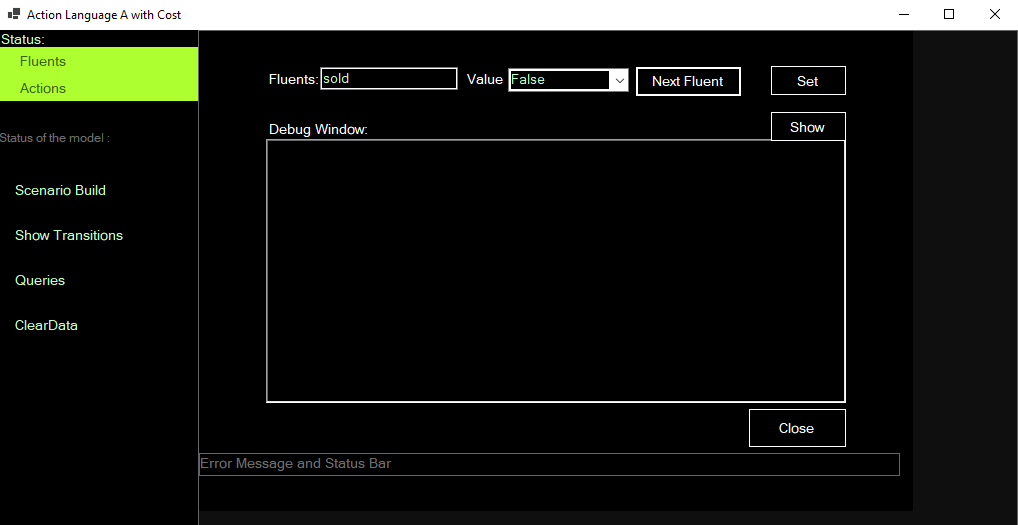
\includegraphics[width=6in,height=3in]{./testImages/Example2/img4.png}
		\label{Figure:f02.4}
		\caption{Set Initial state}
	\end{figure}
	\begin{figure}[H]
		\centering
		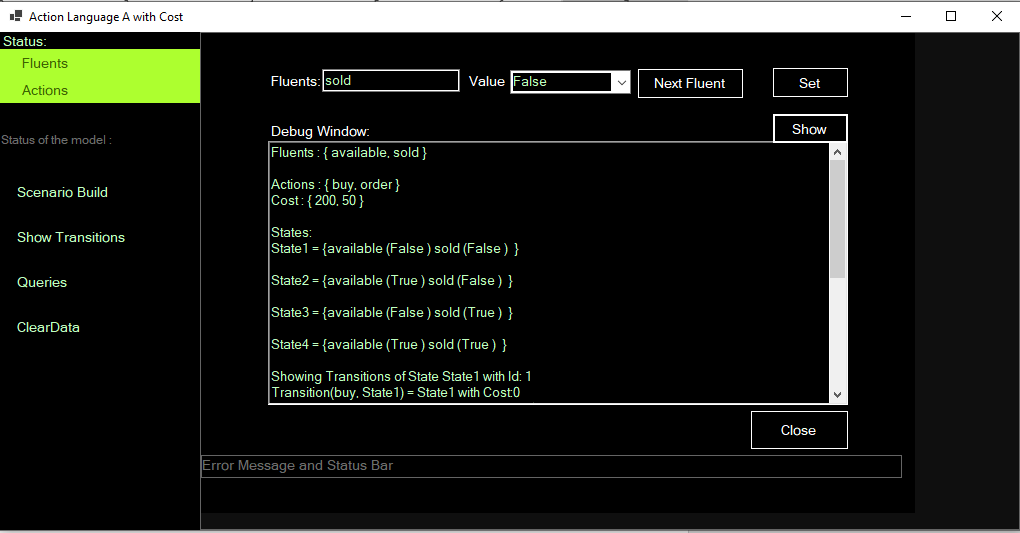
\includegraphics[width=6in,height=3in]{./testImages/Example2/img5.png}
		\label{Figure:f02.5}
		\caption{Show Transitions}
	\end{figure}
		\begin{figure}[H]
		\centering
		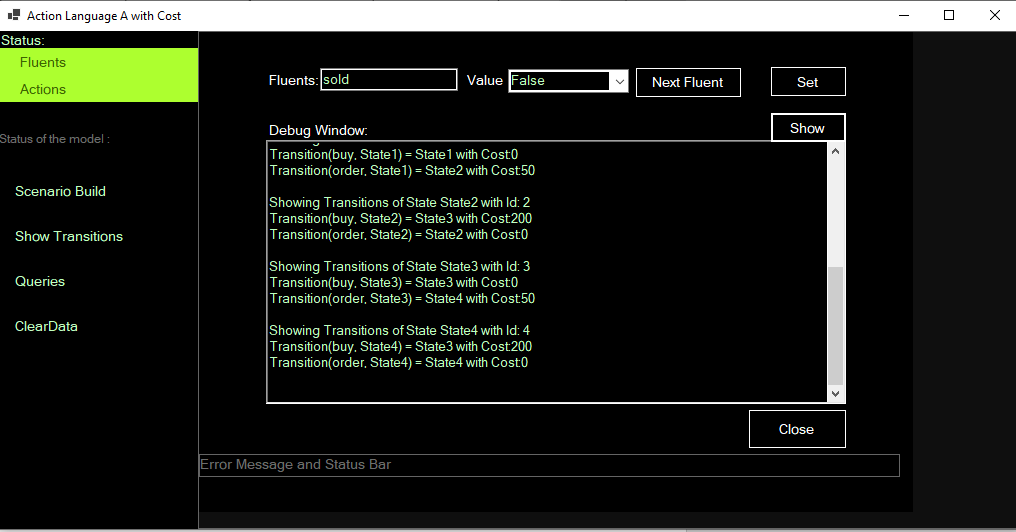
\includegraphics[width=6in,height=3in]{./testImages/Example2/img6.png}
		\label{Figure:f02.6}
		\caption{Show Transition contd..}
	\end{figure}
		\begin{figure}[H]
		\centering
		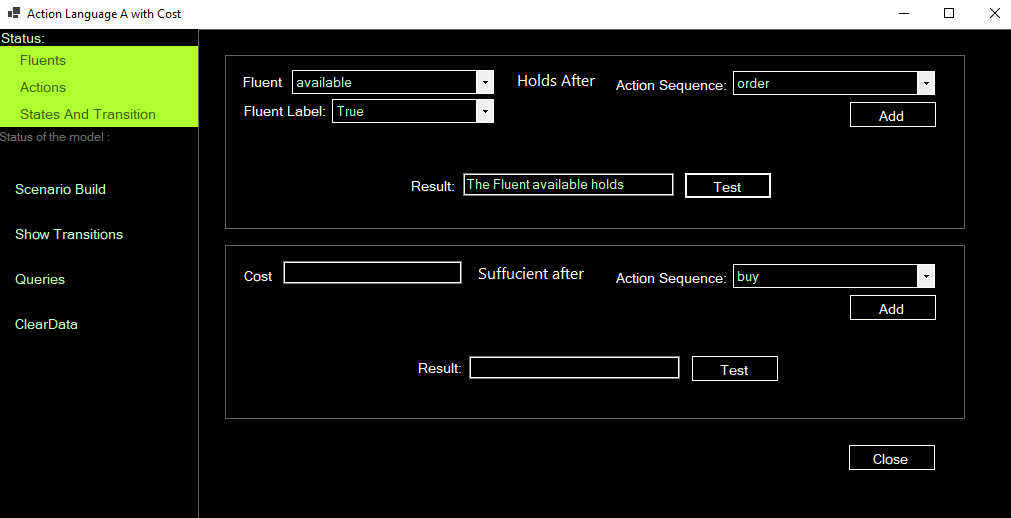
\includegraphics[width=6in,height=3in]{./testImages/Example2/img7.png}
		\label{Figure:f02.7}
		\caption{Queries(Fluents)}
	\end{figure}
	\begin{figure}[H]
		\centering
		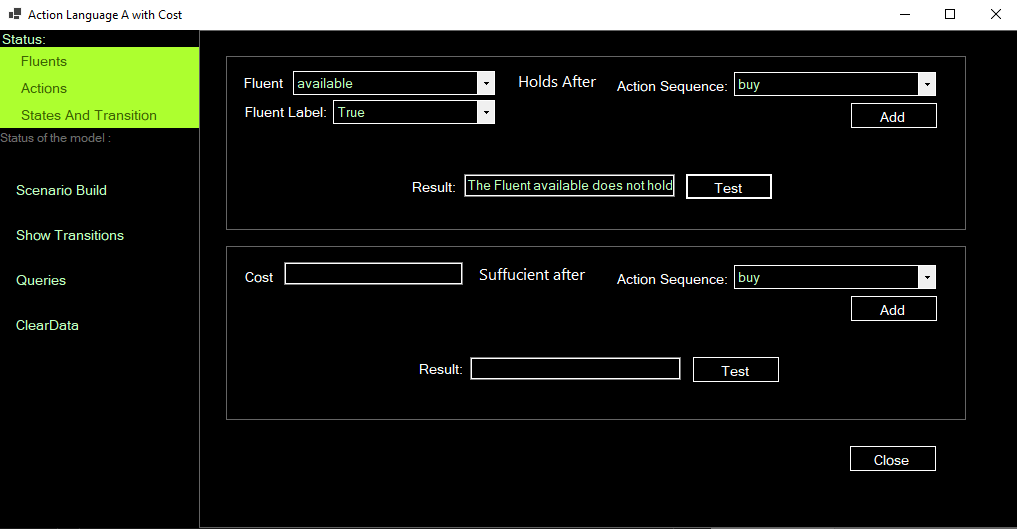
\includegraphics[width=6in,height=3in]{./testImages/Example2/img8.png}
		\label{Figure:f02.8}
		\caption{Queries(Fluents)}
	\end{figure}
	\begin{figure}[H]
		\centering
		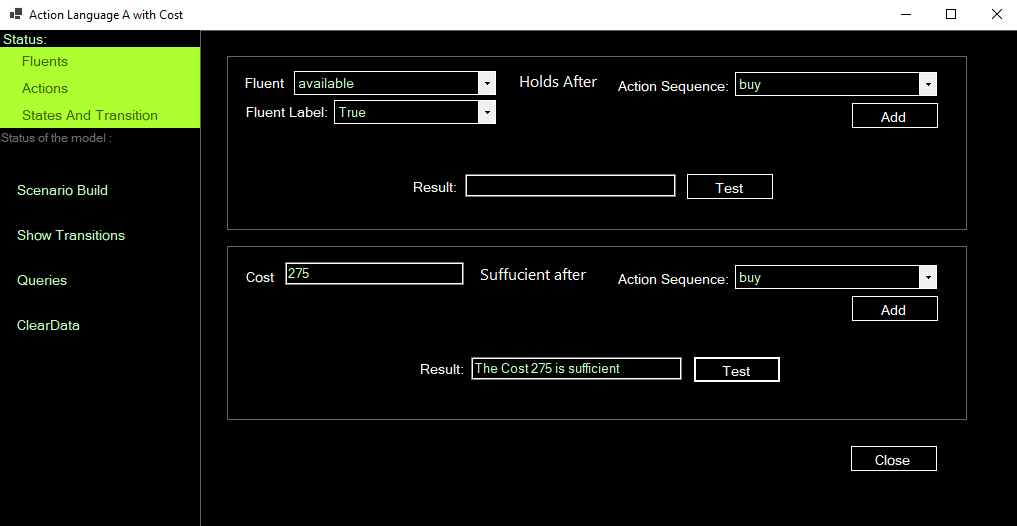
\includegraphics[width=6in,height=3in]{./testImages/Example2/img9.png}
		\label{Figure:f02.9}
		\caption{Queries(Cost)}
	\end{figure}
	\begin{figure}[H]
		\centering
		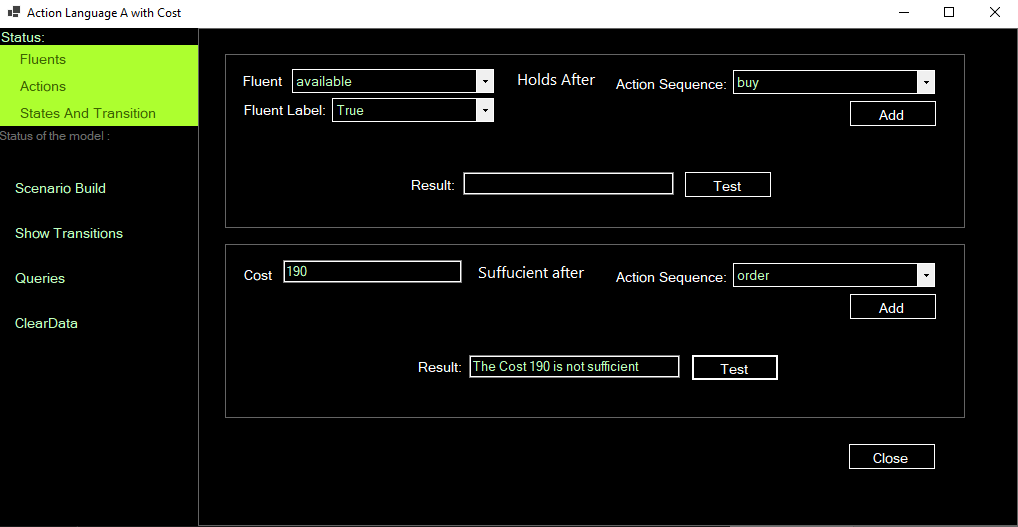
\includegraphics[width=6in,height=3in]{./testImages/Example2/img10.png}
		\label{Figure:f02.10}
		\caption{Queries(Cost)}
	\end{figure}

		

	\subsection{Example 03}
	\subsubsection{Description}\label{par:p103}
	There is a man. He can cook, eat, and play. Cooking makes food cooked. he can eat food if it is cooked. After eating he feels not hungry, and food is not cooked again. He can play. Playing makes him hungry. He just can play if he is not hungry. He just cooks when there is no food is cooked. Initially, he is hungry, and no food is cooked. In terms of energy, eating costs 5, cooking costs 15, playing costs 20.\\
	\\
	\subsubsection{Representation in language}\label{par:p203}
	Fluents: F = \{cooked, hungry\}\\
	Actions: Ac = \{cook, eat, play\}\\
	Costs: K = \{15, 5, 20\}
	\\
	\\
	initially $\neg$cooked;\\
	initially hungry;\\
	cook causes cooked if $\neg$cooked;\\
	cook costs 15;\\
	eat causes $\neg$cooked if cooked;\\
	eat causes $\neg$hungry if cooked;\\
	eat costs 5;\\
	play causes hungry if $\neg$hungry;\\
	play costs 20;\\
	\\
	\subsubsection{Calculation}\label{par:p303}
	$\sum$ = \{$\sigma_{0}$ ,$\sigma_{1}$, $\sigma_{2}$, $\sigma_{3}$\}\\
	\\
	$\sigma_{0}$ = \{$\neg$cooked, hungry\}\\
	$\sigma_{1}$ = \{cooked, hungry\}\\
	$\sigma_{2}$ = \{$\neg$cooked, $\neg$hungry\}\\
	$\sigma_{3}$ = \{cooked, $\neg$hungry\}\\
	\\
	\(  \Psi  \)(eat, $\sigma_{0}$) = $\sigma_{0}$\\
	\(  \Psi  \)(cook, $\sigma_{0}$) = $\sigma_{1}$\\
	\(  \Psi  \)(play, $\sigma_{0}$) = $\sigma_{0}$\\
	\(\Gamma\)(eat, $\sigma_{0}$) = 0\\
	\(\Gamma\)(cook, $\sigma_{0}$) = 15\\
	\(\Gamma\)(play, $\sigma_{0}$) = 0\\
	\\
	\(  \Psi  \)(eat, $\sigma_{1}$) = $\sigma_{2}$\\
	\(  \Psi  \)(cook, $\sigma_{1}$) = $\sigma_{1}$\\
	\(  \Psi  \)(play, $\sigma_{1}$) = $\sigma_{1}$\\
	\(\Gamma\)(eat, $\sigma_{1}$) = 5\\
	\(\Gamma\)(cook, $\sigma_{1}$) = 0\\
	\(\Gamma\)(play, $\sigma_{1}$) = 0\\
	\\
	\(  \Psi  \)(eat, $\sigma_{2}$) = $\sigma_{2}$\\
	\(  \Psi  \)(cook, $\sigma_{2}$) = $\sigma_{3}$\\
	\(  \Psi  \)(play, $\sigma_{2}$) = $\sigma_{0}$\\
	\(\Gamma\)(eat, $\sigma_{2}$) = 0\\
	\(\Gamma\)(cook, $\sigma_{2}$) = 15\\
	\(\Gamma\)(play, $\sigma_{2}$) = 20\\
	\\
	\(  \Psi  \)(eat, $\sigma_{3}$) = $\sigma_{2}$\\
	\(  \Psi  \)(cook, $\sigma_{3}$) = $\sigma_{3}$\\
	\(  \Psi  \)(play, $\sigma_{3}$) = $\sigma_{1}$\\
	\(\Gamma\)(eat, $\sigma_{3}$) = 5\\
	\(\Gamma\)(cook, $\sigma_{3}$) = 0\\
	\(\Gamma\)(play, $\sigma_{3}$) = 20\\
	\\
	\subsubsection{Graph}\label{par:p403}
	\begin{figure}[H]
		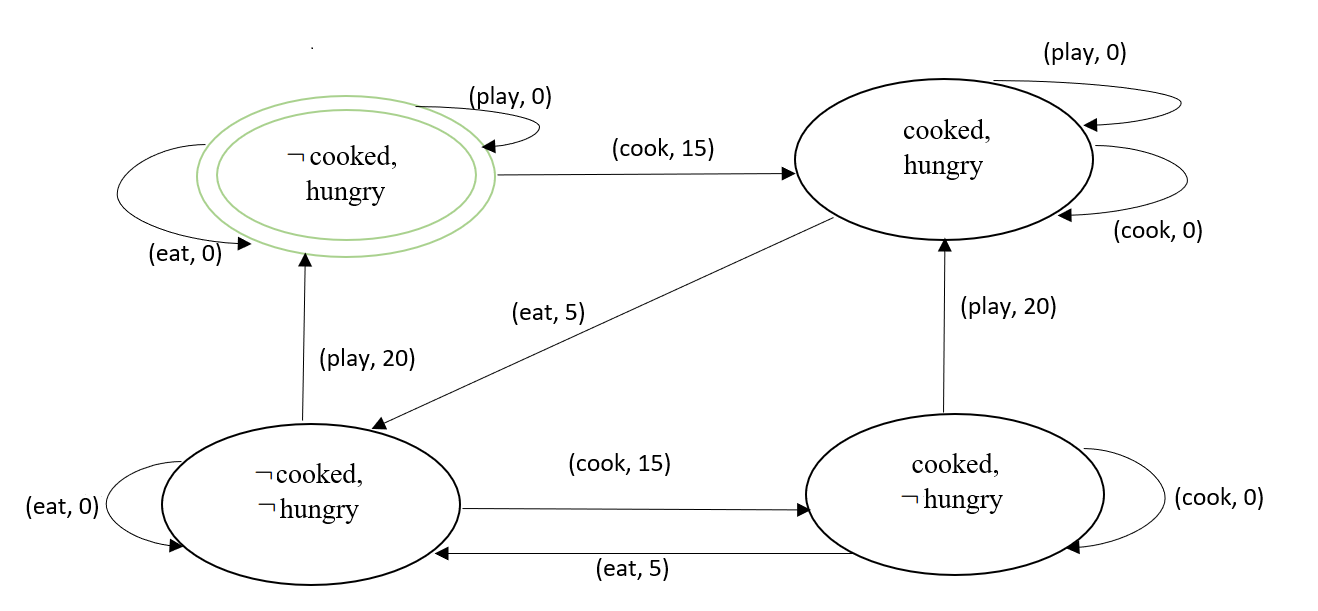
\includegraphics[width=1\linewidth, height=0.3\textheight]{./media/figure01.png}
		\caption{Example 03}
		\label{Figure:f03}
	\end{figure}
	\subsubsection{Queries}
	cooked holds after (play, play, eat, cook): True\\
	cooked holds after (cook, eat play, cook): False\\
	\\
	40 sufficient for (play, cook, eat, cook): True\\
	20 sufficient for (cook, eat, cook, play): False\\
	\subsubsection*{Test Images}\label{par:502}
	\begin{figure}[H]
		\centering
		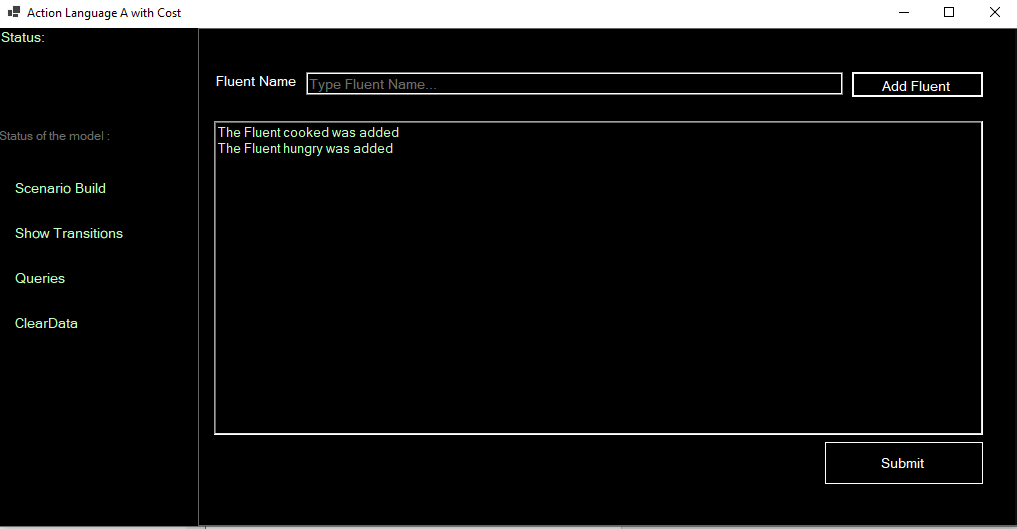
\includegraphics[width=6in,height=3in]{./testImages/Example3/img1.png}
		\label{Figure:f03.1}
		\caption{Add Fluents}
	\end{figure}
	\begin{figure}[H]
		\centering
		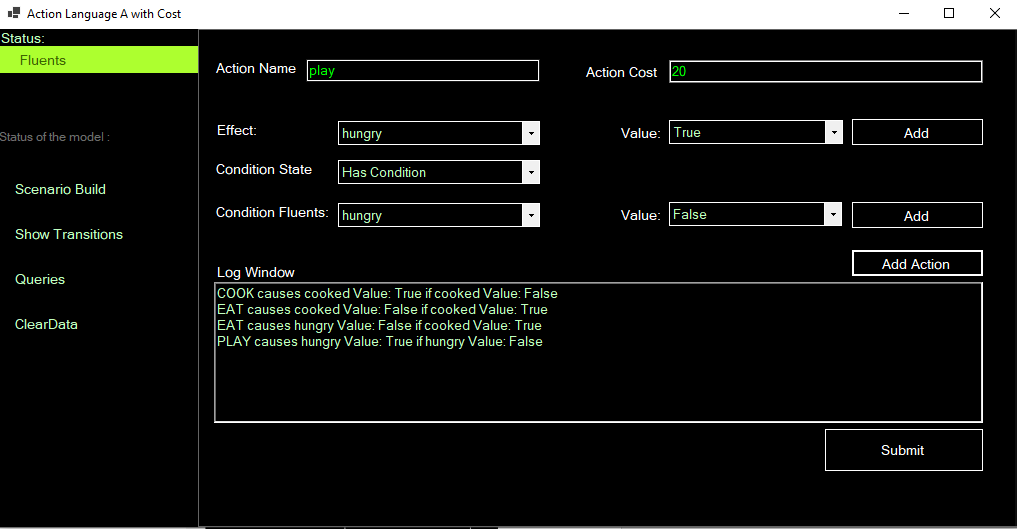
\includegraphics[width=6in,height=3in]{./testImages/Example3/img2.png}
		\label{Figure:f03.2}
		\caption{Add Actions}
	\end{figure}
	\begin{figure}[H]
		\centering
		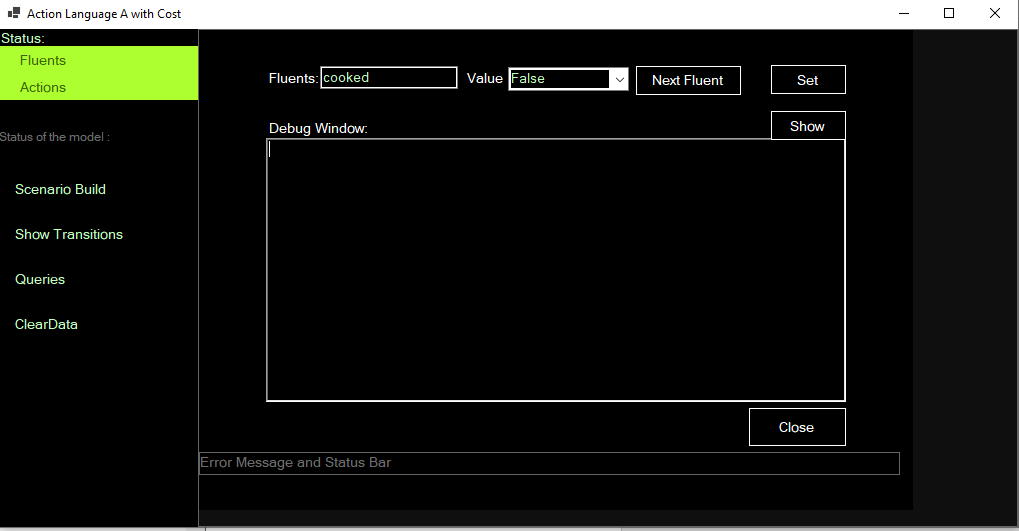
\includegraphics[width=6in,height=3in]{./testImages/Example3/img3.png}
		\label{Figure:f03.3}
		\caption{Set Initial State fluents}
	\end{figure}
	\begin{figure}[H]
		\centering
		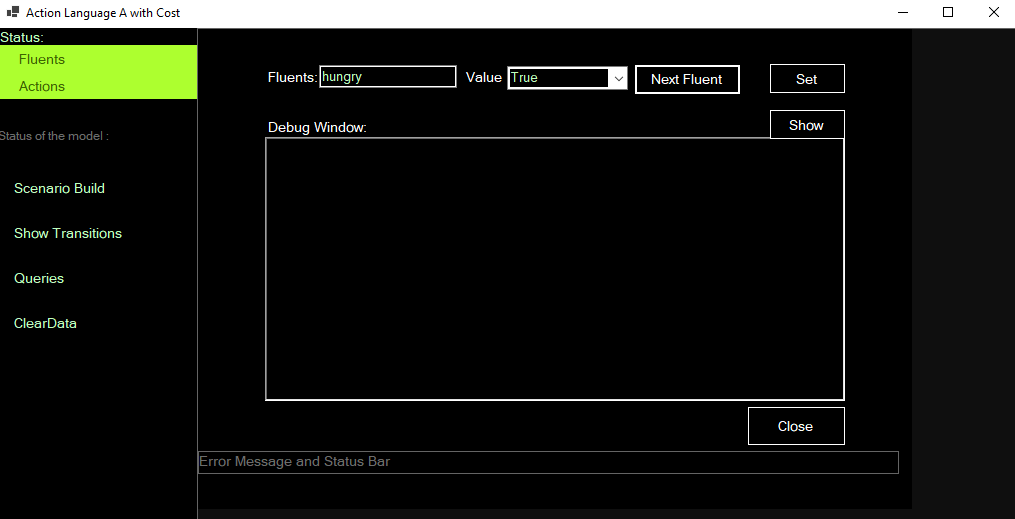
\includegraphics[width=6in,height=3in]{./testImages/Example3/img4.png}
		\label{Figure:f03.4}
		\caption{Set Initial state}
	\end{figure}
	\begin{figure}[H]
		\centering
		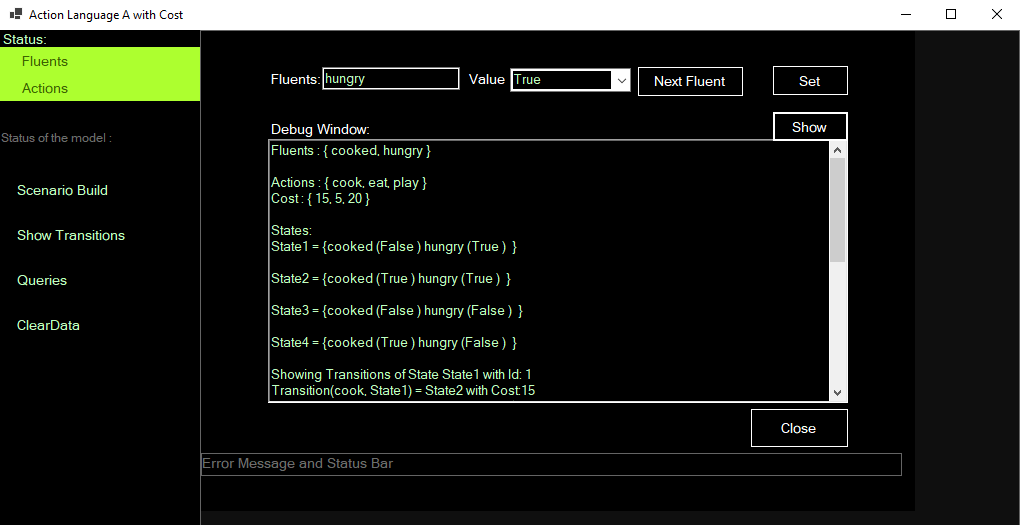
\includegraphics[width=6in,height=3in]{./testImages/Example3/img5.png}
		\label{Figure:f03.5}
		\caption{Show Transitions}
	\end{figure}
		\begin{figure}[H]
		\centering
		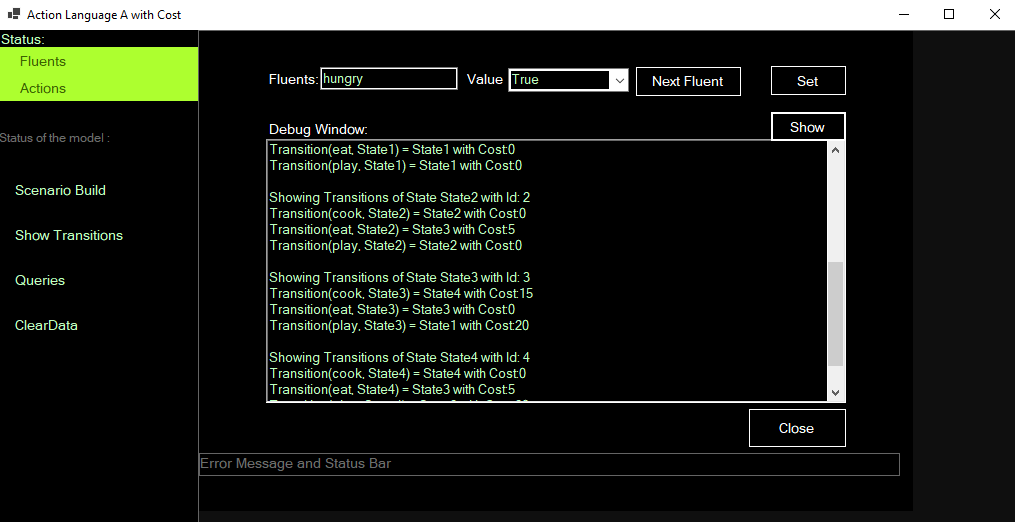
\includegraphics[width=6in,height=3in]{./testImages/Example3/img6.png}
		\label{Figure:f03.6}
		\caption{Show Transitions contd..}
	\end{figure}
		\begin{figure}[H]
		\centering
		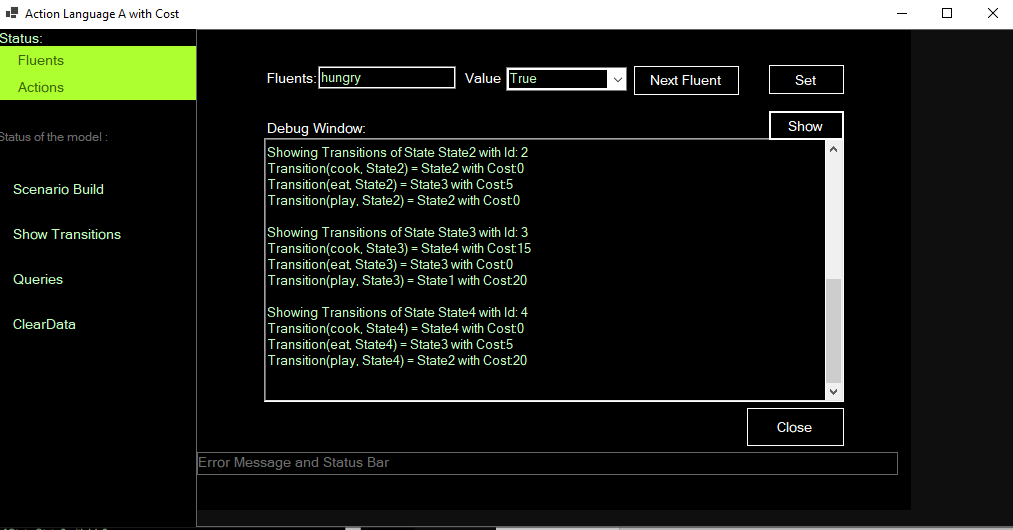
\includegraphics[width=6in,height=3in]{./testImages/Example3/img7.png}
		\label{Figure:f03.7}
		\caption{Show Transitions contd..)}
	\end{figure}
	\begin{figure}[H]
		\centering
		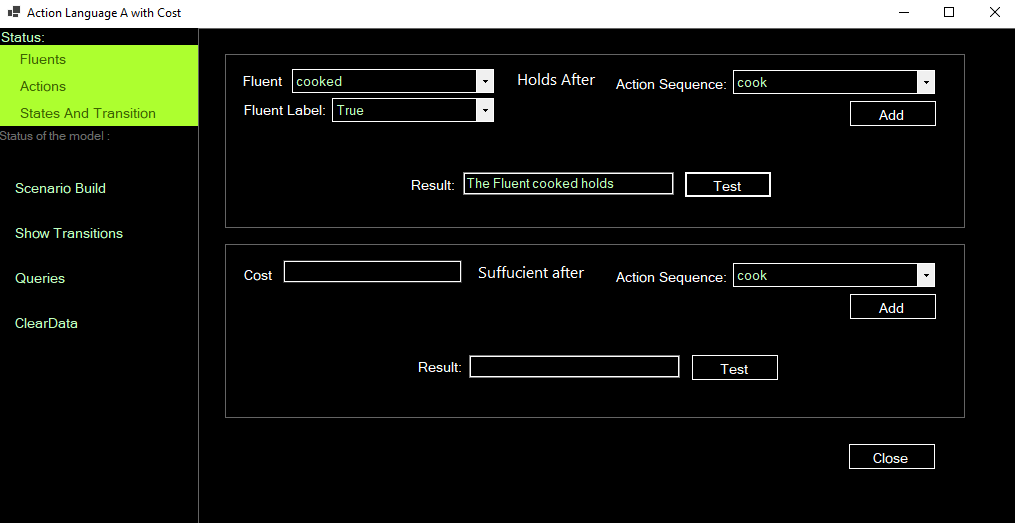
\includegraphics[width=6in,height=3in]{./testImages/Example3/img8.png}
		\label{Figure:f03.8}
		\caption{Queries(Fluents)}
	\end{figure}
	\begin{figure}[H]
		\centering
		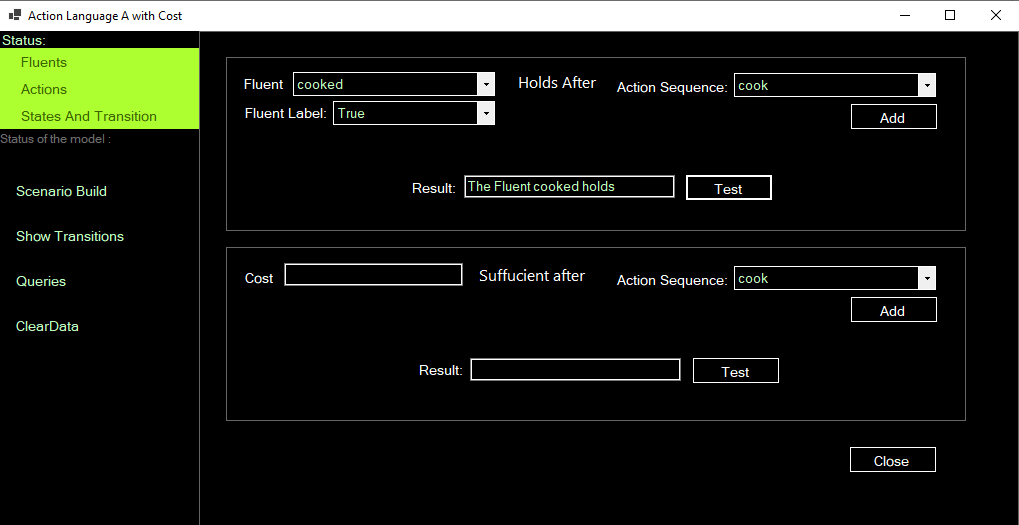
\includegraphics[width=6in,height=3in]{./testImages/Example3/img9.png}
		\label{Figure:f03.9}
		\caption{Queries(Fluents)}
	\end{figure}
	\begin{figure}[H]
		\centering
		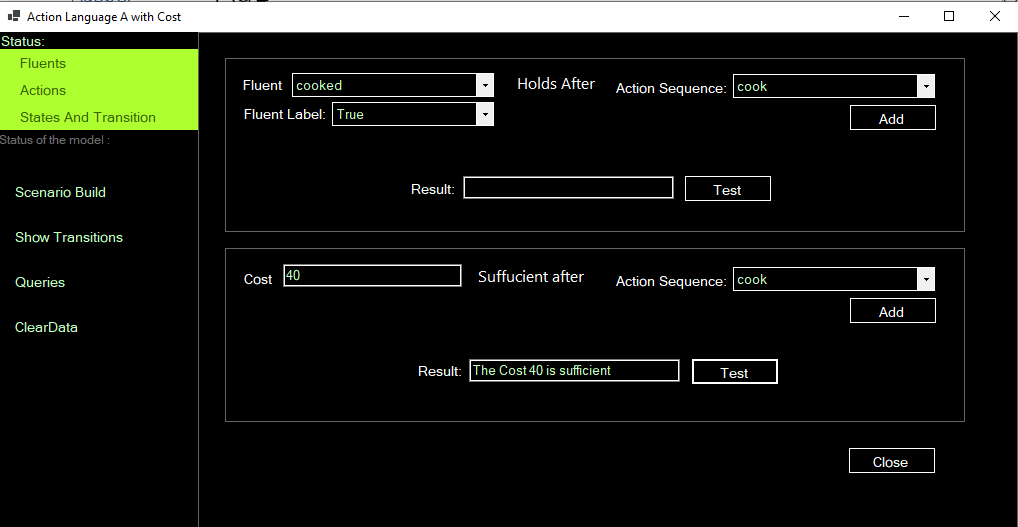
\includegraphics[width=6in,height=3in]{./testImages/Example3/img10.png}
		\label{Figure:f03.10}
		\caption{Queries(Cost)}
	\end{figure}
	\begin{figure}[H]
		\centering
		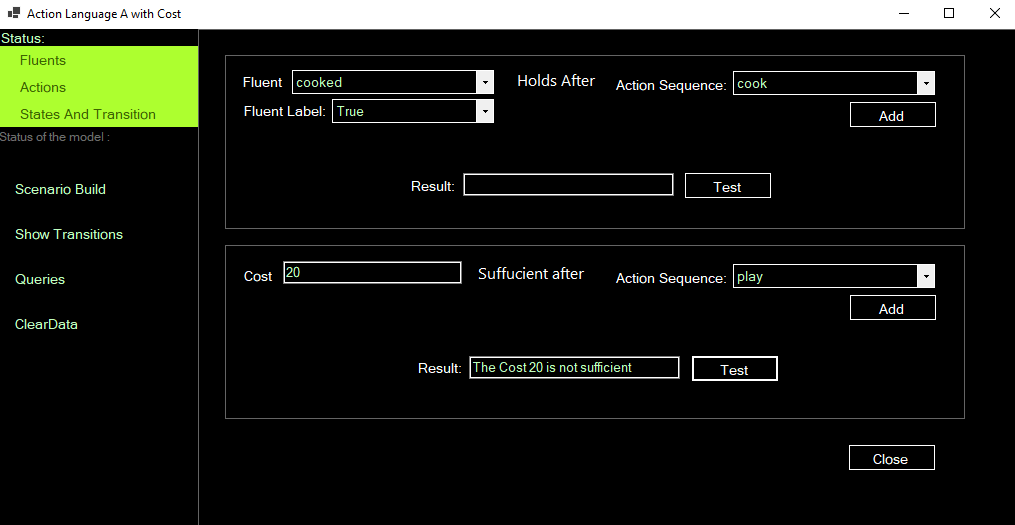
\includegraphics[width=6in,height=3in]{./testImages/Example3/img11.png}
		\label{Figure:f03.11}
		\caption{Queries(Cost)}
	\end{figure}
	\newpage
	\section{Appendix}	
	\begin{appendix}
		\listoffigures
		\listoftables
	\end{appendix}
		 
\end{document}
